\documentclass{standalone}
\usepackage{tikz}
\usetikzlibrary{patterns, positioning}
\usepackage[sfdefault]{ClearSans} %% option 'sfdefault' activates Clear Sans as the default text font
\usepackage[T1]{fontenc}

\begin{document}
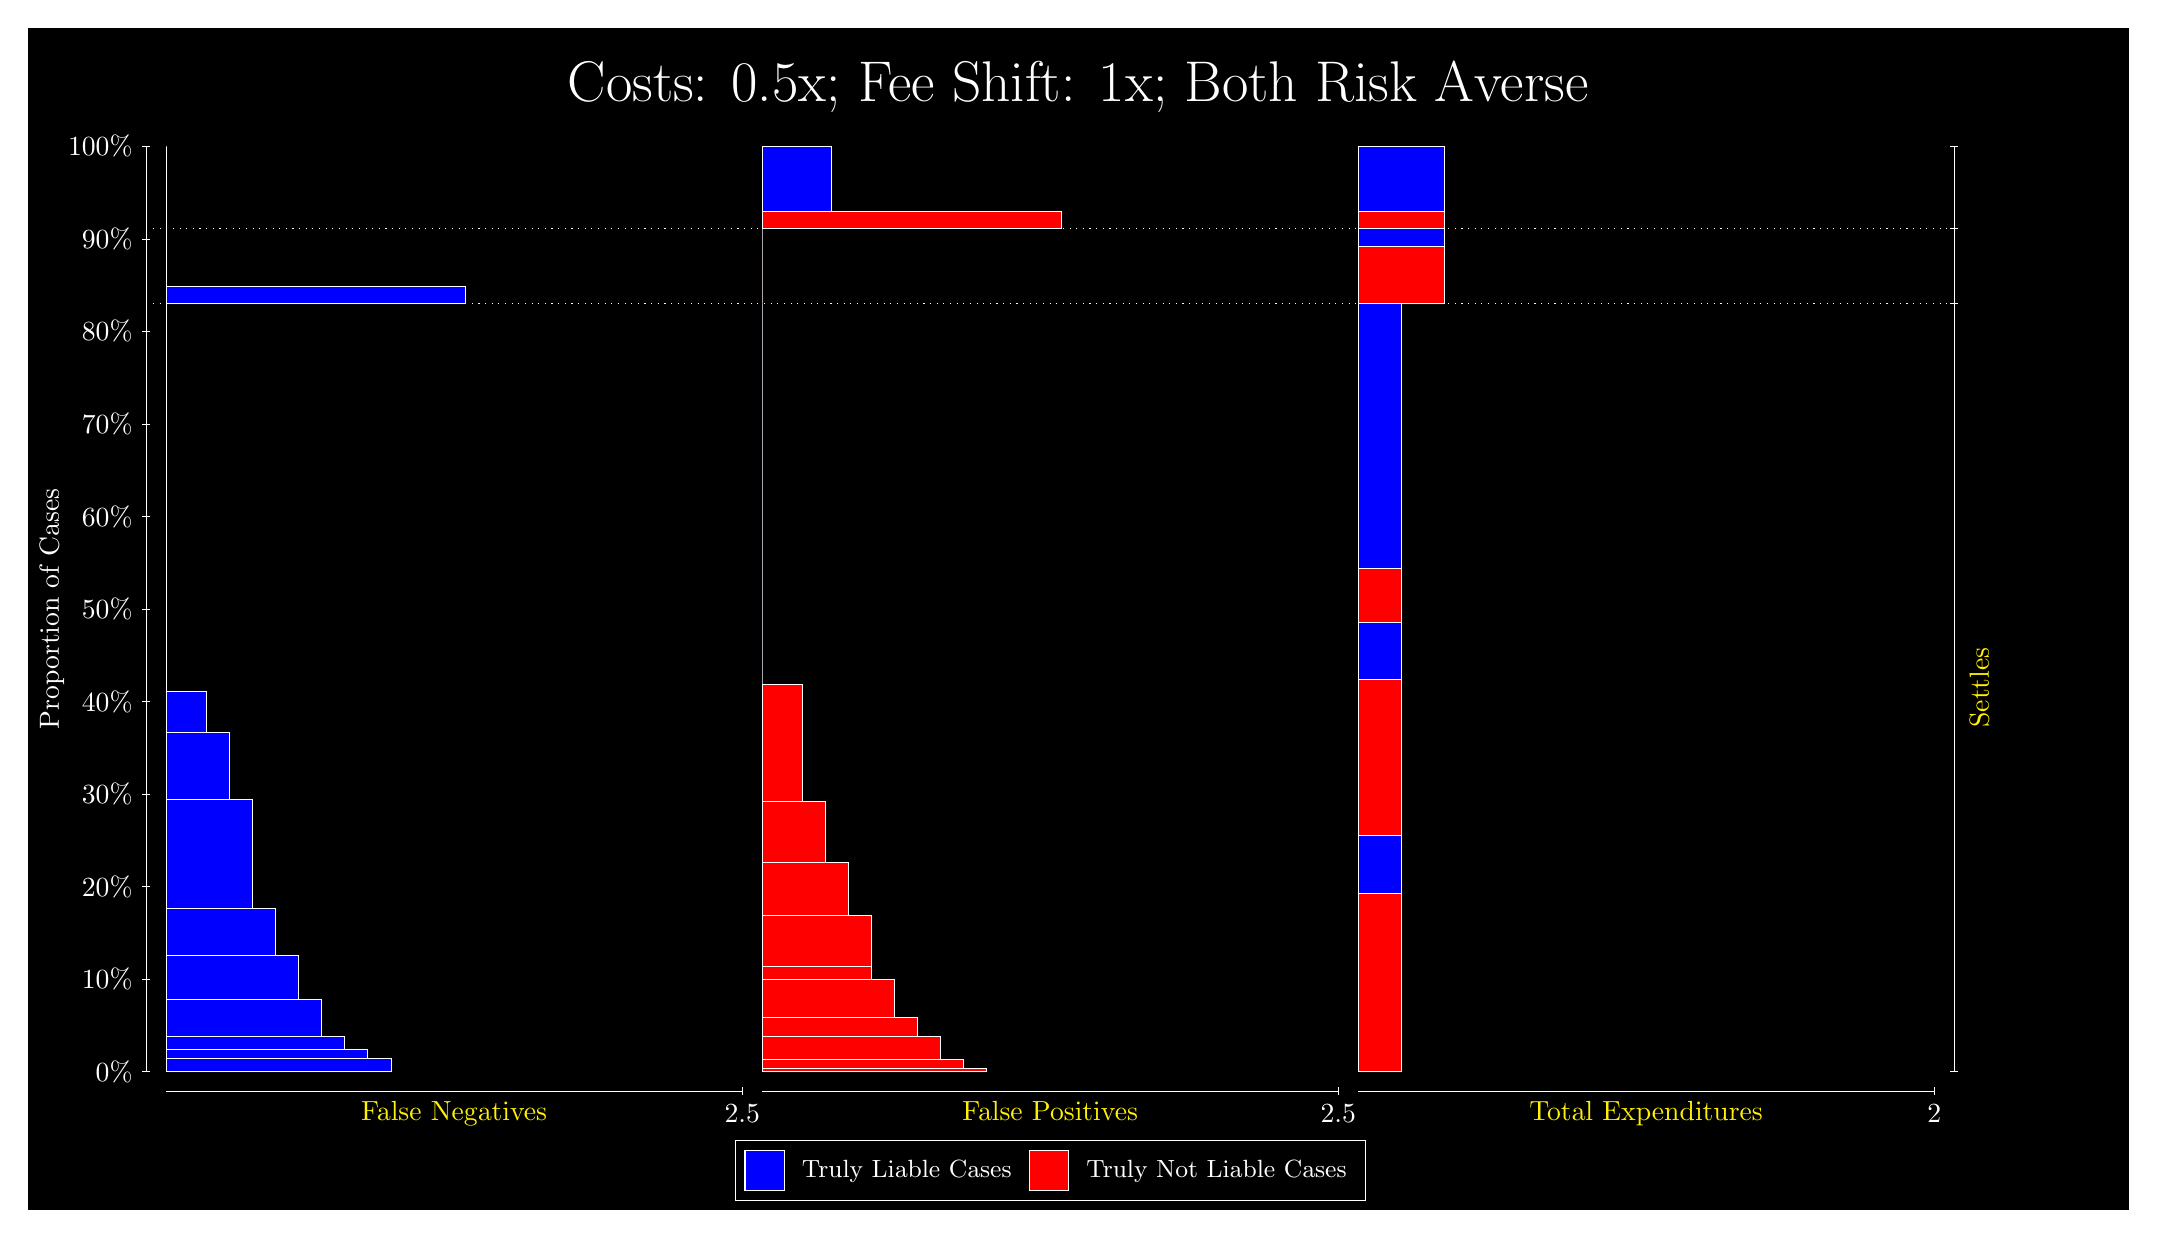
\begin{tikzpicture}
\draw[fill=black] (0,0) rectangle (26.667,15);
\draw[text=white] (0,13.5) rectangle (26.667,15) node[midway] {\huge Costs: 0.5x; Fee Shift: 1x; Both Risk Averse};
\draw[white, very thin] (1.5,1.75) -- (1.5,13.5);
\node[rotate=90, text=white, anchor=center] at (0.3, 7.625) {Proportion of Cases};
\draw[white, very thin] (1.45,1.75) -- (1.55,1.75);
\node[text=white, anchor=east] at (1.45, 1.75) {0\%};
\draw[white, very thin] (1.45,2.925) -- (1.55,2.925);
\node[text=white, anchor=east] at (1.45, 2.925) {10\%};
\draw[white, very thin] (1.45,4.1) -- (1.55,4.1);
\node[text=white, anchor=east] at (1.45, 4.1) {20\%};
\draw[white, very thin] (1.45,5.275) -- (1.55,5.275);
\node[text=white, anchor=east] at (1.45, 5.275) {30\%};
\draw[white, very thin] (1.45,6.45) -- (1.55,6.45);
\node[text=white, anchor=east] at (1.45, 6.45) {40\%};
\draw[white, very thin] (1.45,7.625) -- (1.55,7.625);
\node[text=white, anchor=east] at (1.45, 7.625) {50\%};
\draw[white, very thin] (1.45,8.8) -- (1.55,8.8);
\node[text=white, anchor=east] at (1.45, 8.8) {60\%};
\draw[white, very thin] (1.45,9.975) -- (1.55,9.975);
\node[text=white, anchor=east] at (1.45, 9.975) {70\%};
\draw[white, very thin] (1.45,11.15) -- (1.55,11.15);
\node[text=white, anchor=east] at (1.45, 11.15) {80\%};
\draw[white, very thin] (1.45,12.325) -- (1.55,12.325);
\node[text=white, anchor=east] at (1.45, 12.325) {90\%};
\draw[white, very thin] (1.45,13.5) -- (1.55,13.5);
\node[text=white, anchor=east] at (1.45, 13.5) {100\%};

\draw[white, very thin] (24.457,1.75) -- (24.457,13.5);
\draw[white, very thin] (24.407,1.75) -- (24.507,1.75);
\node[anchor=west] at (24.407, 1.75) {};
\draw[white, very thin] (24.407,11.506) -- (24.507,11.506);
\node[anchor=west] at (24.407, 11.506) {};
\draw[white, very thin] (24.407,12.458) -- (24.507,12.458);
\node[anchor=west] at (24.407, 12.458) {};
\draw[white, very thin] (24.407,13.5) -- (24.507,13.5);
\node[anchor=west] at (24.407, 13.5) {};

\draw[white, very thin, fill=blue] (1.75,1.75) rectangle (4.6044,1.9164);
\draw[white, very thin, fill=blue] (1.75,1.9164) rectangle (4.3116,2.0371);
\draw[white, very thin, fill=blue] (1.75,2.0371) rectangle (4.0188,2.1943);
\draw[white, very thin, fill=blue] (1.75,2.1943) rectangle (3.7261,2.6616);
\draw[white, very thin, fill=blue] (1.75,2.6616) rectangle (3.4333,3.2208);
\draw[white, very thin, fill=blue] (1.75,3.2208) rectangle (3.1406,3.8196);
\draw[white, very thin, fill=blue] (1.75,3.8196) rectangle (2.8478,5.21);
\draw[white, very thin, fill=blue] (1.75,5.21) rectangle (2.5551,6.0523);
\draw[white, very thin, fill=blue] (1.75,6.0523) rectangle (2.2623,6.5838);
\draw[white, very thin, fill=red] (1.75,6.5838) rectangle (1.75,11.506);
\draw[white, very thin, fill=blue] (1.75,11.506) rectangle (5.5558,11.728);
\draw[white, very thin, fill=red] (1.75,11.728) rectangle (1.75,12.458);
\draw[white, very thin, fill=red] (1.75,12.458) rectangle (1.75,12.681);
\draw[white, very thin, fill=blue] (1.75,12.681) rectangle (1.75,13.5);
\draw[white, very thin, fill=red] (9.3189,1.75) rectangle (12.173,1.7939);
\draw[white, very thin, fill=red] (9.3189,1.7939) rectangle (11.88,1.8995);
\draw[white, very thin, fill=red] (9.3189,1.8995) rectangle (11.588,2.1932);
\draw[white, very thin, fill=red] (9.3189,2.1932) rectangle (11.295,2.4401);
\draw[white, very thin, fill=red] (9.3189,2.4401) rectangle (11.002,2.926);
\draw[white, very thin, fill=red] (9.3189,2.926) rectangle (10.709,3.0815);
\draw[white, very thin, fill=red] (9.3189,3.0815) rectangle (10.709,3.735);
\draw[white, very thin, fill=red] (9.3189,3.735) rectangle (10.417,4.4118);
\draw[white, very thin, fill=red] (9.3189,4.4118) rectangle (10.124,5.1839);
\draw[white, very thin, fill=red] (9.3189,5.1839) rectangle (9.8312,6.6721);
\draw[white, very thin, fill=blue] (9.3189,6.6721) rectangle (9.3189,11.506);
\draw[white, very thin, fill=red] (9.3189,11.506) rectangle (9.3189,12.236);
\draw[white, very thin, fill=blue] (9.3189,12.236) rectangle (9.3189,12.458);
\draw[white, very thin, fill=red] (9.3189,12.458) rectangle (13.125,12.681);
\draw[white, very thin, fill=blue] (9.3189,12.681) rectangle (10.197,13.5);
\draw[white, very thin, fill=red] (16.888,1.75) rectangle (17.437,4.0079);
\draw[white, very thin, fill=blue] (16.888,4.0079) rectangle (17.437,4.7531);
\draw[white, very thin, fill=red] (16.888,4.7531) rectangle (17.437,6.7272);
\draw[white, very thin, fill=blue] (16.888,6.7272) rectangle (17.437,7.4528);
\draw[white, very thin, fill=red] (16.888,7.4528) rectangle (17.437,8.1429);
\draw[white, very thin, fill=blue] (16.888,8.1429) rectangle (17.437,11.506);
\draw[white, very thin, fill=red] (16.888,11.506) rectangle (17.986,12.236);
\draw[white, very thin, fill=blue] (16.888,12.236) rectangle (17.986,12.458);
\draw[white, very thin, fill=red] (16.888,12.458) rectangle (17.986,12.681);
\draw[white, very thin, fill=blue] (16.888,12.681) rectangle (17.986,13.5);
\draw[white, dotted] (1.5,11.506) -- (24.457,11.506);
\draw[white, dotted] (1.5,12.458) -- (24.457,12.458);
\draw[white, very thin] (1.75,1.5) -- (9.0689,1.5);
\node[text=yellow, anchor=north] at (5.4094, 1.5) {False Negatives};
\draw[white, very thin] (9.0689,1.45) -- (9.0689,1.55);
\node[text=white, anchor=north] at (9.0689, 1.45) {2.5};

\draw[white, very thin] (9.3189,1.5) -- (16.638,1.5);
\node[text=yellow, anchor=north] at (12.978, 1.5) {False Positives};
\draw[white, very thin] (16.638,1.45) -- (16.638,1.55);
\node[text=white, anchor=north] at (16.638, 1.45) {2.5};

\draw[white, very thin] (16.888,1.5) -- (24.207,1.5);
\node[text=yellow, anchor=north] at (20.547, 1.5) {Total Expenditures};
\draw[white, very thin] (24.207,1.45) -- (24.207,1.55);
\node[text=white, anchor=north] at (24.207, 1.45) {2};

\node[text=yellow, centered, rotate=90] at (24.777, 6.6279) {Settles};



\draw (12.978300999999998,1.5) node[draw=none] (baseCoordinate) {};
\begin{scope}[align=center]
        \matrix[scale=0.5, draw=white, below=0.5cm of baseCoordinate, nodes={draw}, column sep=0.1cm]{
            \node[rectangle, draw, minimum width=0.5cm, minimum height=0.5cm, fill=blue] {}; &
            \node[draw=none, font=\small, text=white] (B) {Truly Liable Cases}; &
            \node[rectangle, draw, minimum width=0.5cm, minimum height=0.5cm, fill=red] {}; &
            \node[draw=none, font=\small, text=white] (B) {Truly Not Liable Cases}; \\
            };
\end{scope}

\end{tikzpicture}
\end{document}